% Preamble
\documentclass[12pt, a4paper]{article}
\title{\emph{Best Books for Human\\Emotions} \& \emph{Disorders}}
\author{Written by Volunteers}
\date{July 12, 2021}

% Packages
\usepackage{xcolor}
\usepackage{caption}
\usepackage[utf8]{inputenc}
\usepackage{hyperref}
\usepackage{graphicx}
\graphicspath{{images/}}

% Body
\begin{document}
\maketitle
\begin{enumerate}

\item Social Skills
\item Generalized Anxiety Disorder
\item Social Anxiety Disorder \& Shyness
\item Overthinking
\item Jealousy
\item Self-awareness
\item Self-consciousness
\item Happiness
\item Paranoia
\item Revenge
\item Self-confidence / Self-esteem
\item False Self-confidence / Self-esteem
\item Addiction
\item OCD
\item Perfectionism
\item Child Abuse
\item Painful Past
\item Panic Attack
\item Self-harm / Self-injury
\item Suicide
\item Trauma
\item Post Traumatic Stress Disorder
\item Shizoaffective
\item Shizophernia
\item Hallucinations
\item Delusional Disorder
\item Major Depressive Disorder
\item Dysthymia
\item Bipolar Disorder

\end{enumerate}

\begin{center}
	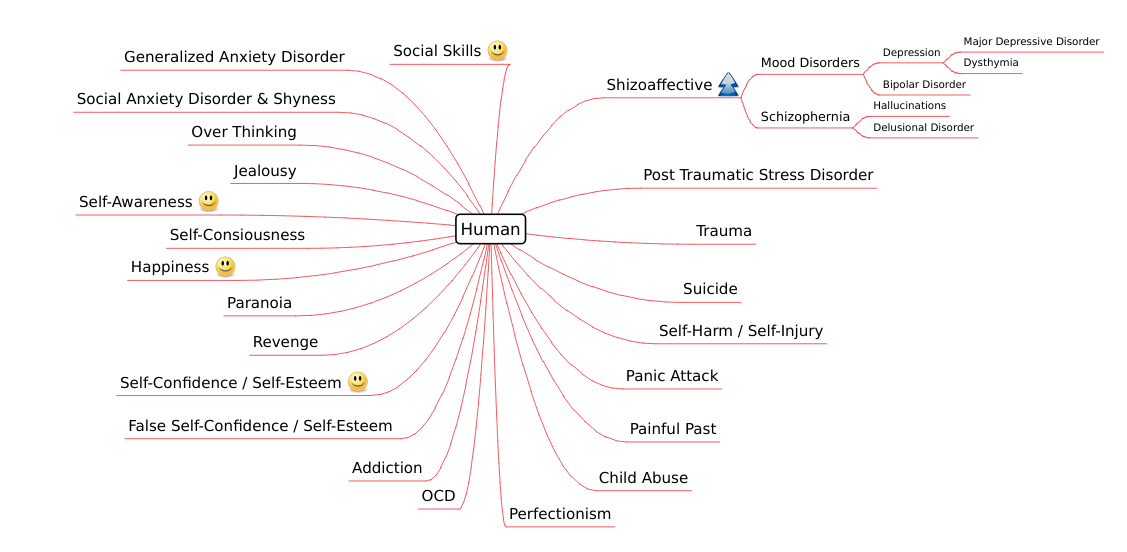
\includegraphics[scale=0.43]{human.png}
\end{center}

\newpage

\begin{large}
\paragraph{}
If you want to contribute, read these considerations:

\begin{enumerate}

\item The author should have a PhD degree in related topic
\item The author should be an expert in that field
\item The author's methods must be applicable

\end{enumerate}

\end{large}

\newpage

% Social Skills
\section*{\scalebox{1.4}{\emph{Social Skills}}}
\subsubsection*{\emph{The Social Skills Guide Book}}
\subsubsection*{\emph{How to Win Friends and Influence People}}
\subsubsection*{\emph{Conversationally Speaking}}
\subsubsection*{\emph{How to Speak, How to Listen}\\}

\subsection*{\scalebox{1.3}{\emph{* Additional *}}}
\subsubsection*{\emph{Improve your Social Skills}\\}


% Generalized Anxiety Disorder
\section*{\scalebox{1.4}{\emph{Generalized Anxiety Disorder}}}
\subsubsection*{\scalebox{0.9}{\emph{Generalized Anxiety Disorder Work Book: A Comprehensive CBT Guide}}}
\subsubsection*{\emph{Rewire your Anxious Brain}\\}

\subsection*{\scalebox{1.3}{\emph{* Additional *}}}
\subsubsection*{\scalebox{0.9}{\emph{Cognitive Behavioral Anxiety Disorder Treatment for Generalized}}}
\subsubsection*{\scalebox{0.9}{\emph{The Anxiety and Worry Workbook: The Cognitive Behavioural Solution}}}
\subsubsection*{\scalebox{0.9}{\emph{Generalized Anxiety Disorder: Advances in Research and Practice}}\\}


% Social Anxiety Disorder & Shyness
\section*{\scalebox{1.4}{\emph{Social Anxiety Disorder} \& \emph{Shyness}}}
\subsubsection*{\emph{The Shyness} \& \emph{Social Anxiety Workbook}}
\subsubsection*{\emph{Overcoming Social Anxiety} \& \emph{Shyness}\\}

% Overthinking
\section*{\scalebox{1.4}{\emph{Overthinking}}}
\subsubsection*{\emph{The Worry Trick}}
\subsubsection*{\emph{Soundtracks: The Suprising Solution to Overthinking}\\}

\newpage

% Self-confidence / Self-esteem
\section*{\scalebox{1.4}{\emph{Self-confidence / Self-esteem}}}
\subsubsection*{\emph{The Confidence Gap}}
\subsubsection*{\emph{The Self-confidence Workbook}\\}

\subsection*{\scalebox{1.3}{\emph{* Additional *}}}
\subsubsection*{\emph{Self-esteem: A Proven Program of Cognitive Technique}}
\subsubsection*{\emph{How to be yourself}}







\end{document}
